\subsection{Plant Scaling}
\label{sec:plantscale}

Plant scaling is a rather important section as it dictats the flowrates and storage requirements the plant has to adhere to, in order to satisfy consumer demand.

The plant simulation was used with demand and wind data fed into the function blocks (see Figure \ref{fig:global}). A simulation was run to obtain an estimate on the material and energy requirements for the plant.

The material balance for the first design iteration was produced in Figure \ref{flowsheettbl}.

These data were used to scale other components and to demonstrate that with approximate efficiency values from literature that this is a feasible project (see sections \ref{} and \ref{}).

A rather startling conclusion from this analysis is that the ESS stores far less energy than was orginally expected.
The windspeeds in Maui are sufficiently high all-year-round to satisfy the bulk of consumer demand.

\begin{figure}[tbh]
    \centering
    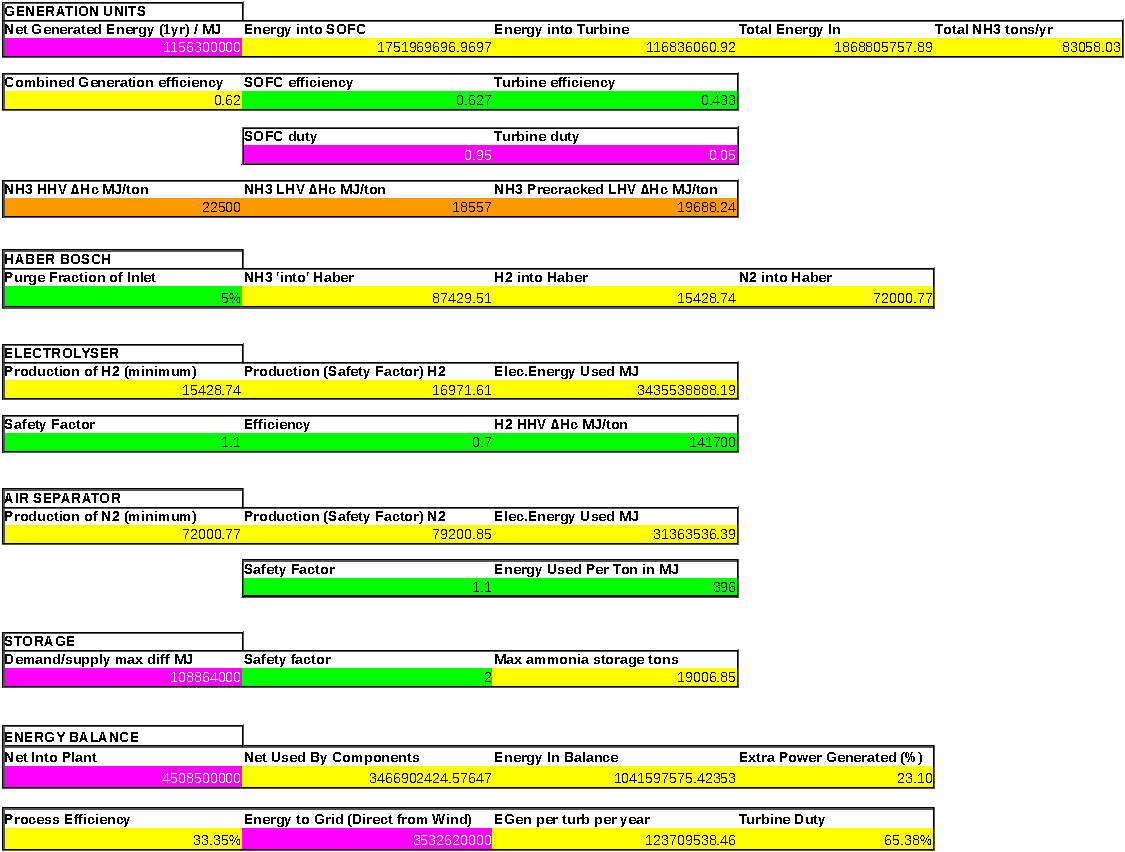
\includegraphics[scale=0.9]{images/flowtable.pdf}
    \caption{An approximate material balance flowsheet using efficiency factors from all components, demand and wind data.}
    \label{flowsheettbl}
\end{figure}